\chapter{Generative models}


\begin{description}
    \item[Generative task] \marginnote{Generative task}
        Given the training data $\{ x^{(i)} \}$, learn the distribution of the data so that a model can sample new examples:
        \[ \hat{x}^{(i)} \sim p_\text{gen}(x; \matr{\theta}) \]

        \begin{figure}[H]
            \centering
            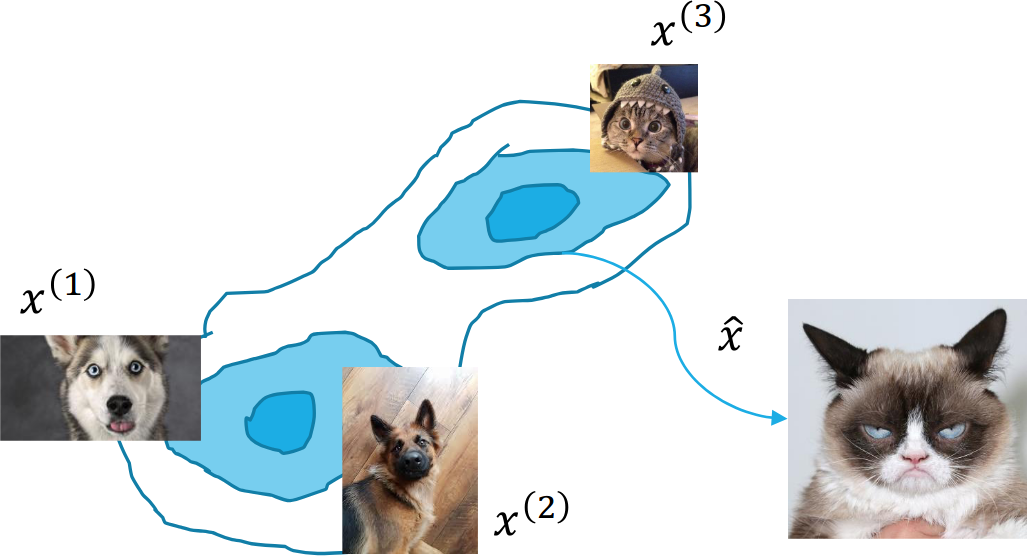
\includegraphics[width=0.4\linewidth]{./img/generative_task.png}
        \end{figure}

        \begin{remark}
            Generative tasks are hard as natural images lay on a low dimensional subspace (i.e., only a tiny subset of all the possible RGB images makes sense).

            \begin{figure}[H]
                \centering
                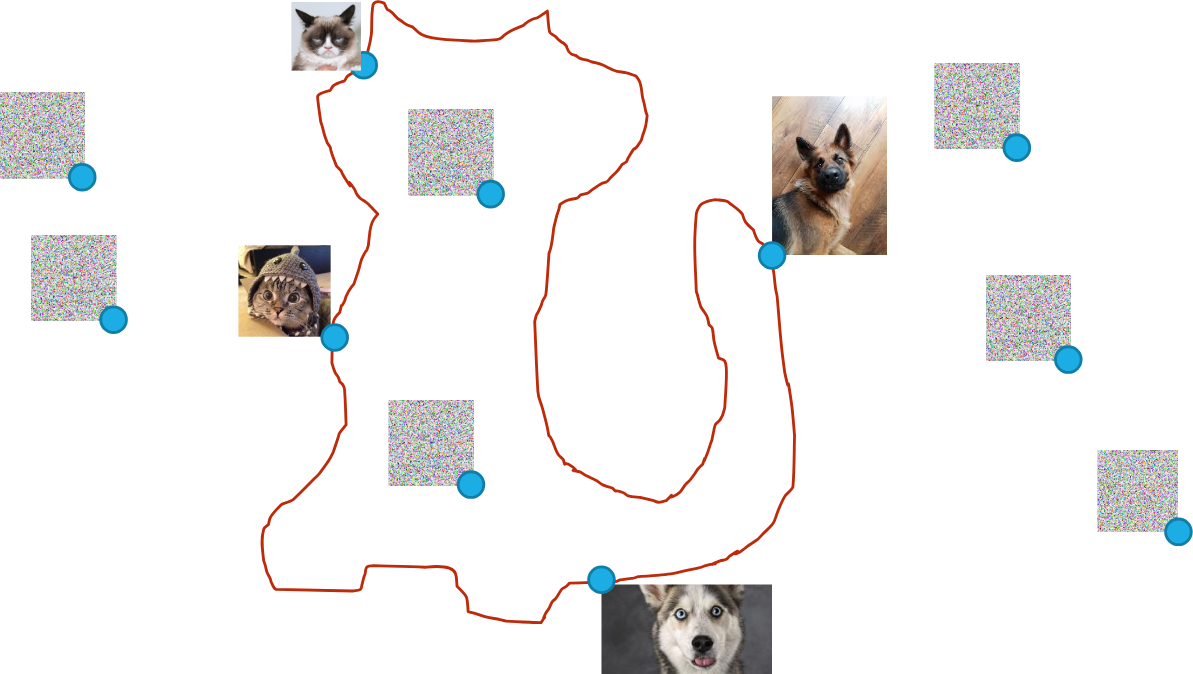
\includegraphics[width=0.6\linewidth]{./img/image_manifold.png}
            \end{figure}
        \end{remark}

    \item[Latent vector] \marginnote{Latent vector}
        Low-dimensional representation to encode an image.

        \begin{example}
            Face expression depends on 42 muscles. A latent representation for different poses of a face can be represented with a 42-dimensional vector.
        \end{example}

        It is assumed that the factors of a latent vector are independent or mildly correlated, and can be sampled from a known distribution.

    \item[Generative model] \marginnote{Generative model}
        Model that takes as input a latent representation and maps it into an output image.
        \begin{figure}[H]
            \centering
            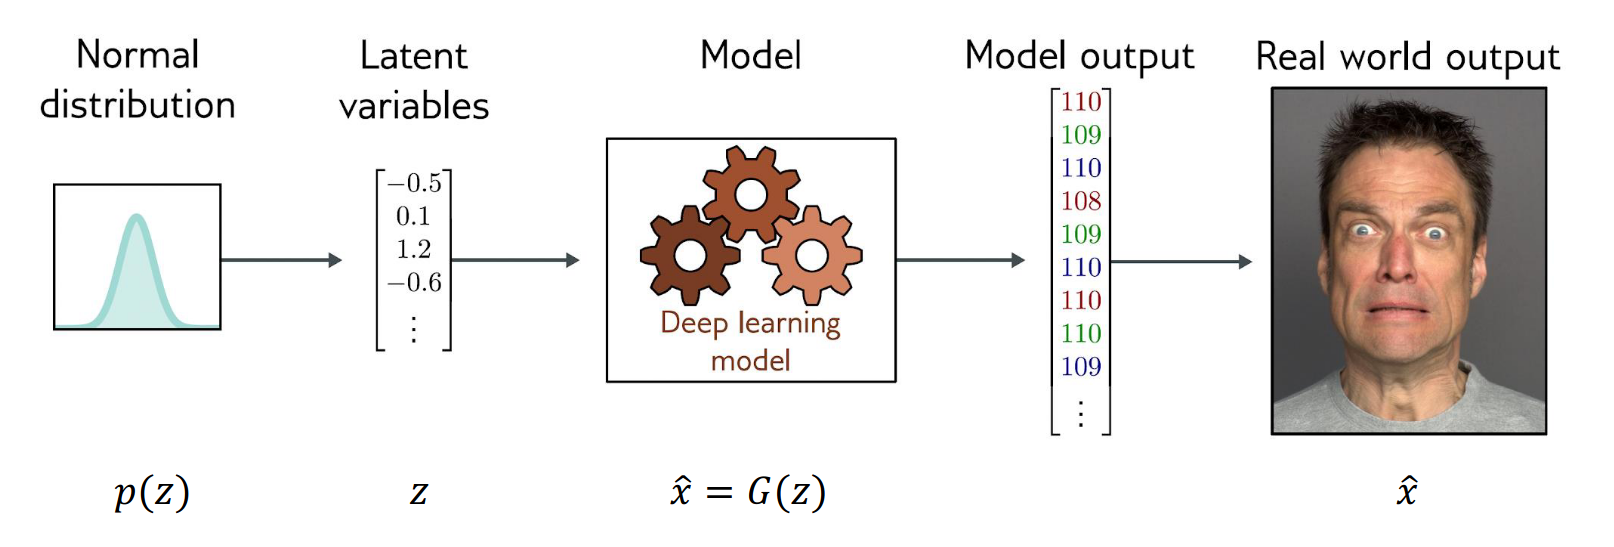
\includegraphics[width=0.7\linewidth]{./img/latent_for_generation.png}
        \end{figure}

        \begin{remark}
            An ideal generative model should have the following properties:
            \begin{itemize}
                \item Be computationally efficient when sampling.
                \item Produce high-quality samples.
                \item Represent the entire training distribution.
                \item Produce a plausible output from any latent input. Smooth changes to the input should be reflected on the output.
                \item Have a disentangled latent space (i.e., changing a dimension of the latent space corresponds to interpretable changes in the output image).
                \item Have the possibility to calculate the probability of the produced images (when the model is probabilistic). 
            \end{itemize}
        \end{remark}
\end{description}



\section{Metrics}

\begin{description}
    \item[Expectation/Expected value] \marginnote{Expectation/Expected value}
        Informally, it is the generalization of the weighted average:
        \[ 
            \mathbb{E}_{x \sim p}[ f(\cdot) ] = \sum_{x \in \mathbb{X}} p(x) f(x) 
            \qquad
            \mathbb{E}_{x \sim p}[ f(\cdot) ] = \int_{x \in \mathbb{X}} p(x) f(x) \,dx
        \]

        \begin{description}
            \item[Monte Carlo approximation] \marginnote{Monte Carlo approximation}
                Approximation for expectation using $N$ i.i.d. samples drawn from $p(x)$:
                \[ \mathbb{E}_{x \sim p}[f(\cdot)] \approx \frac{1}{N} \sum_{x_i \sim p(x)} f(x_i) \]
        \end{description}

    \item[Self-information] \marginnote{Self-information}
        Given a probability mass function of an event, the self-information of an event $x$ is defined as:
        \[ I(x) = -\log_b(p(x)) = \log_b\left( \frac{1}{p(x)} \right) \]
        Intuitively, it can be seen as a measure of surprise.

        \begin{remark}
            If $b = 2$, self-information is measured in bits. If $b = e$, it is measured in natural unit of information ($nat$).
        \end{remark}

        \begin{example}
            Consider the toss of a fair coin. The self-information for the outcomes are:
            \[ I(\texttt{heads}) = I(\texttt{tails}) = \log_2\left( \frac{1}{0.5} \right) = 1 \text{ bit} \]
            If the coin is loaded toward tails with probability:
            \[ 
                \prob{\texttt{heads}} = 0.05 
                \qquad 
                \prob{\texttt{heads}} = 0.95 
            \]
            The self-information is:
            \[ 
                I(\texttt{heads}) = \log_2\left( \frac{1}{0.05} \right) = 4.31 \text{ bits}
                \qquad
                I(\texttt{tails}) = \log_2\left( \frac{1}{0.95} \right) = 0.07 \text{ bits}
            \]
        \end{example}

    \item[Entropy] \marginnote{Entropy}
        Expected value of the self-information of a probability mass function:
        \[ H(p(\cdot)) = \mathbb{E}_{x \sim p} \left[ - \log(p(\cdot)) \right] \approx -\sum_{x \in \mathbb{X}} p(x) \log(p(x)) \]
        Intuitively, it measures the average surprise of a distribution.
        
        \begin{example}
            Consider the distribution of a fair, loaded, and constant coin. We have that:
            \begin{descriptionlist}
                \item[Maximum entropy] $H(p_\text{fair}(\cdot)) = 0.5 \log(2) + 0.5 \log(2) = \log(2)$
                \item[Low entropy] $H(p_\text{loaded}(\cdot)) = 0.05 \cdot 4.32 + 0.95 \cdot 0.07 = 0.28$
                \item[Minimum entropy] $H(p_\text{constant}(\cdot)) = 0 + 1 \cdot 0 = 0$
            \end{descriptionlist}
        \end{example}

    \item[Kullback-Leibler (KL) divergence] \marginnote{Kullback-Leibler (KL) divergence}
        Distance between probability distributions:
        \[ 
            \begin{split}
                D_\text{KL}(p || q) &= \mathbb{E}_{x \sim p(x)}\left[ \log(p(x)) - \log(q(x)) \right] = \mathbb{E}_{x \sim p(x)} \left[ \log\left( \frac{p(x)}{q(x)} \right) \right] \\ 
                &\approx \sum_{x \in \mathbb{X}} \left( p(x) \log\left( \frac{p(x)}{q(x)} \right) \right) 
            \end{split}
        \]

        \begin{remark}
            KL divergence only samples from one of the distributions. Therefore, it is not symmetric (i.e., it is not a metric).
        \end{remark}

        \begin{remark}
            KL divergence goes to infinity if $q(x) = 0$ and $p(x) \neq 0$.
        \end{remark}

        \begin{example}
            Consider the following cases of a coin toss:
            \begin{table}[H]
                \centering
                \begin{tabular}{c|c|c}
                    \toprule
                    & Other distribution is loaded & Other distribution is constant \\
                    \midrule
                    $p$ is fair & 
                        $0.5\log\left(\frac{0.5}{0.05}\right) + 0.5\log\left(\frac{0.5}{0.95}\right) = 0.83$ & 
                        $0.5\log\left(\frac{0.5}{0}\right) + 0.5\log\left(\frac{0.5}{1}\right) = +\infty$ \\
                    $q$ is fair & 
                        $0.05\log\left(\frac{0.05}{0.5}\right) + 0.95\log\left(\frac{0.95}{0.5}\right) = 0.49$ &
                        $0\log\left(\frac{0}{0.5}\right) + 1\log\left(\frac{1}{0.5}\right) = 0.69$ \\
                    \bottomrule
                \end{tabular}
            \end{table}
        \end{example}

    \item[Jensen-Shannon (JS) divergence] \marginnote{Jensen-Shannon (JS) divergence}
        Variation of KL divergence to make it symmetric and bounded:
        \[ [0, \log_b(2)] \ni D_\text{JS}(p || q) = \frac{1}{2} D_\text{KL}\left( p || \frac{p+q}{2} \right) + \frac{1}{2} D_\text{KL}\left( q || \frac{p+q}{2} \right) \]

        \begin{remark}
            JS divergence has the highest value when $p$ and $q$ are disjoint (i.e., $p(x) > 0 \Rightarrow q(x) = 0$ or vice versa).
        \end{remark}

        \begin{remark}
            JS divergence is symmetric and respects the triangle inequality.
        \end{remark}
\end{description}


\subsection{Inception score}

\begin{description}
    \item[Inception score (IS)] \marginnote{Inception score (IS)}
        Given a generator and a pre-trained image classifier, Inception score assesses that:
        \begin{itemize}
            \item The generated images are classified by the classifier with a high confidence (i.e., $p_\text{cls}(y | x)$ should have low entropy).
            \item The generated images cover all the classes handled by the classifier (i.e., $p_\text{cls}(y)$ should have high entropy).
        \end{itemize}
        
        Inception score is computed as:
        \[ 
            \begin{split}
                [1, C] \ni IS &= \exp\left( \mathbb{E}_{x_i \sim p_\text{gen}(x)}\Big[ D_\text{KL}\big( p_\text{cls}(y | x_i) \,||\, p_\text{cls}(y) \big) \Big] \right) \\
                &= \exp\left( H(p_\text{cls}(y)) - \mathbb{E}_{x_i \sim p_\text{gen}(x)} \Big[ H(p_\text{cls}(y | x_i)) \Big] \right)
            \end{split}
        \]
        where $p_\text{cls}(y)$ is computed through Monte Carlo approximation:
        \[ 
            p_\text{cls}(y) = \mathbb{E}_{x \sim p_\text{gen}}\left[ p_\text{cls}(y | x) \right]
            \approx \frac{1}{N} \sum_{x_i \sim p_\text{gen}(x)} p_\text{cls}(y | x_i)
        \]

        \begin{remark}
            Inception score has the following problems:
            \begin{itemize}
                \item It uses the Monte Carlo approximation and requires a large sample size.
                \item It is sensitive to the performance of the classifier.
                \item It does not measure generation diversity within a class.
            \end{itemize}
        \end{remark}

        \begin{figure}[H]
            \centering
            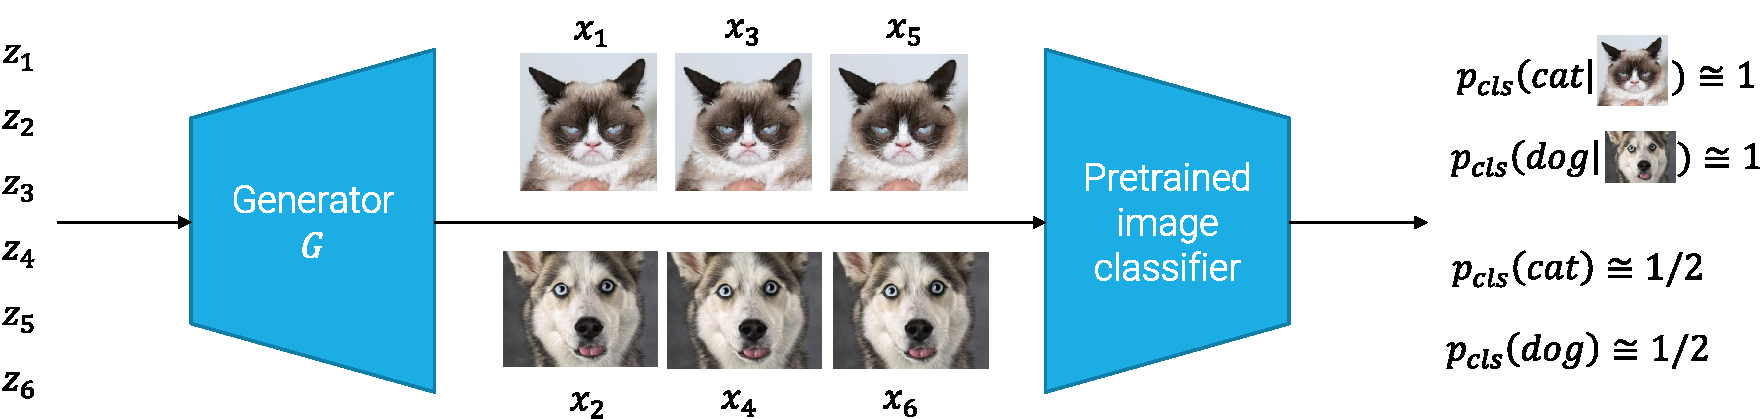
\includegraphics[width=0.8\linewidth]{./img/_inception_score.pdf}
        \end{figure}
\end{description}


\subsection{Fréchet Inception distance}

\begin{description}
    \item[Earth mover's distance (EMD)] \marginnote{Earth mover's distance (EMD)}
        Given two discrete distributions $p$ and $q$, EMD measures the ``work'' needed to match $p$ and $q$ by considering the amount of mass to move and the distance between bins.

        \begin{figure}[H]
            \centering
            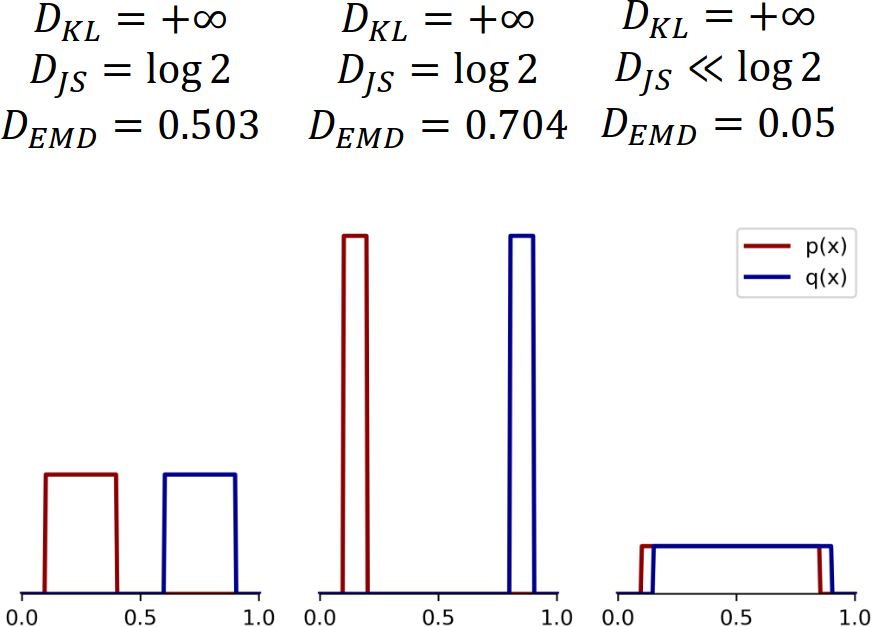
\includegraphics[width=0.4\linewidth]{./img/earth_mover.png}
            \caption{
                \parbox[t]{0.8\linewidth}{
                    Three cases of density functions distance. The distributions in the first case are closer than the second one. In the third case, they are mostly overlapping.
                }
            }
        \end{figure}

        Earth mover's distance is formulated as a linear programming problem:
        \[ 
            \begin{split}
                D_\text{EMD}(p || q) = \min_{\matr{P}}\left[ \sum_{i, j} \matr{P}_{i, j} |i-j| \right] \\
                \begin{split}
                    \text{subject to}& \sum_{i} \matr{P}_{i, j} = p(i) \,\land \\
                        &\sum_j \matr{P}_{i,j} = q(j) \,\land \\
                        &\matr{P}_{i,j} \geq 0
                \end{split}
            \end{split}
        \]
        where $\matr{P}$ is the transport plan such that $\matr{P}_{i,j}$ indicates the amount of mass to move from bin $i$ (of $p$) to bin $j$ (of $q$).

        \begin{figure}[H]
            \centering
            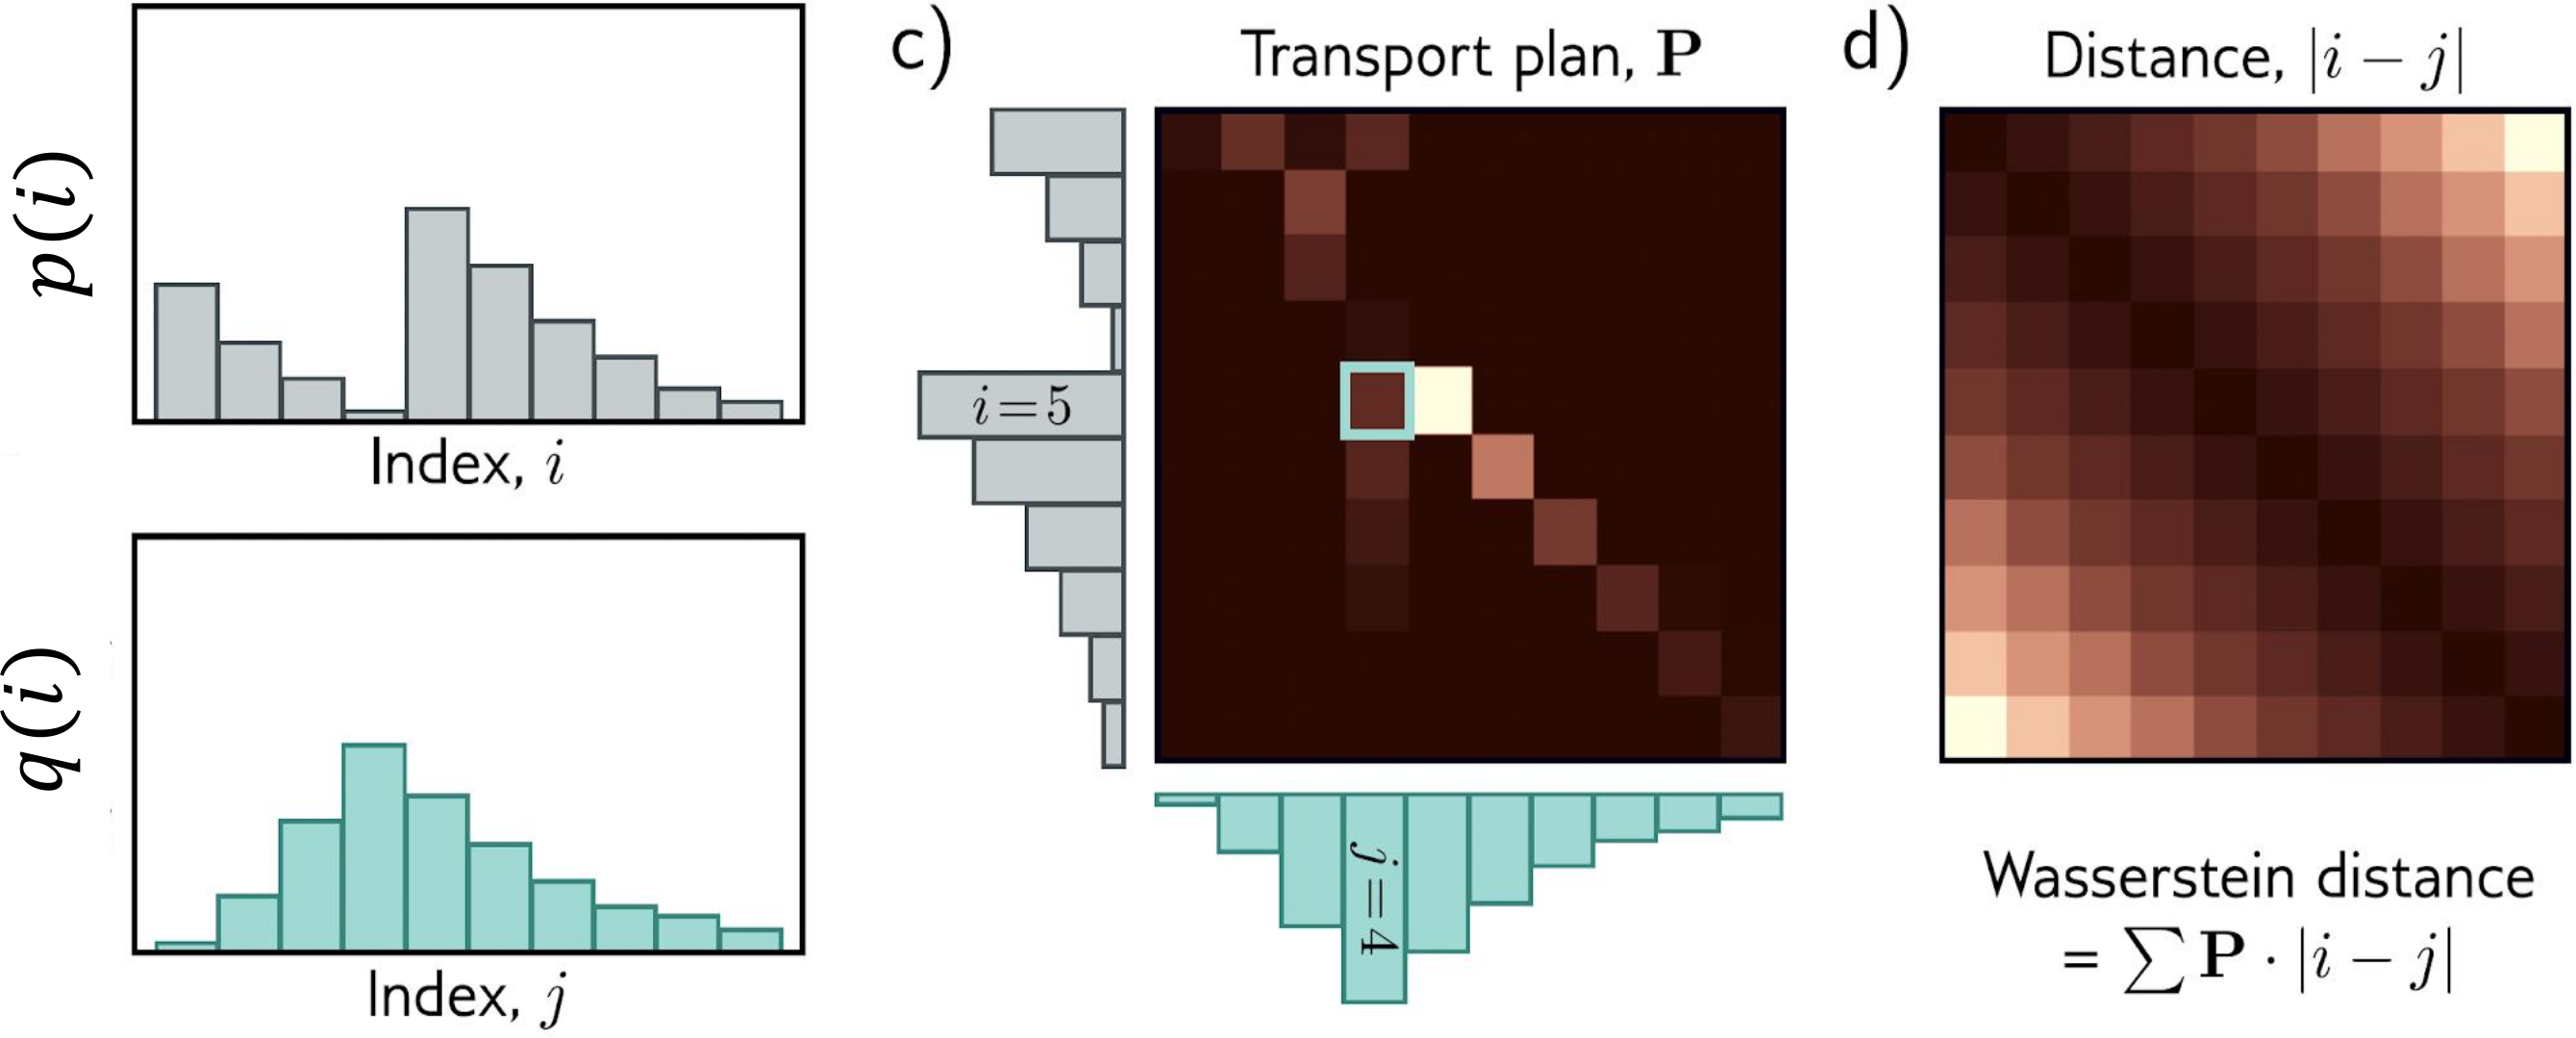
\includegraphics[width=0.6\linewidth]{./img/earth_mover_plan.png}
        \end{figure}


    \item[Fréchet Inception distance (FID)] \marginnote{Fréchet Inception distance (FID)}
        \begin{remark}
            In the continuous case, EMD is computed using the Fréchet distance. Applying it as-is has two problems:
            \begin{itemize}
                \item Comparing pixels is not effective.
                \item The distribution of the generated images cannot be analytically determined.
            \end{itemize} 
        \end{remark}

        Fréchet Inception distance is based on two ideas:
        \begin{itemize}
            \item Use the embedding (Inception-v3) of an image instead of pixels.
            \item Assume that the embedding space is a multi-variate Gaussian.
        \end{itemize}
        Given the Gaussians fitted on the embeddings of the real images $\mathcal{N}(x; \mu_r, \Sigma_r)$ and the embeddings of the generated images $\mathcal{N}(x; \mu_g, \Sigma_g)$, FID is computed as:
        \[ 
            D_\text{FR}^2\left[ \mathcal{N}(x; \mu_r, \Sigma_r) || \mathcal{N}(x; \mu_g, \Sigma_g) \right] = \Vert \mu_g - \mu_r \Vert^2_2 + \text{tr}\left( \Sigma_r + \Sigma_g - 2\sqrt{\Sigma_r \Sigma_g} \right)
        \]
    
    \begin{remark}
        FID accounts for both realism and diversity (FID grows if one of the two distribution is more diverse than the other) both across and within classes. However:
        \begin{itemize}
            \item It is sensitive to the pre-trained feature extractor (but it is more robust than Inception score).
            \item It is not possible to distinguish in the final score whether realism or diversity is the problem.
        \end{itemize}
    \end{remark}
\end{description}


\subsection{Manifold precision/recall}

\begin{description}
    \item[Manifold precision] \marginnote{Manifold precision}
        Fraction of generated images that fall into the real data manifold (i.e., realism).

    \item[Manifold recall] \marginnote{Manifold recall}
        Fraction of real images that fall into the generator manifold (i.e., diversity).
\end{description}

\begin{remark}
    These metrics are computed in the embedding space of the images. The manifold is approximated with a hypersphere centered on each embedding with a radius proportional to the distance to the $k$-th nearest neighbor.
\end{remark}

\begin{figure}[H]
    \centering
    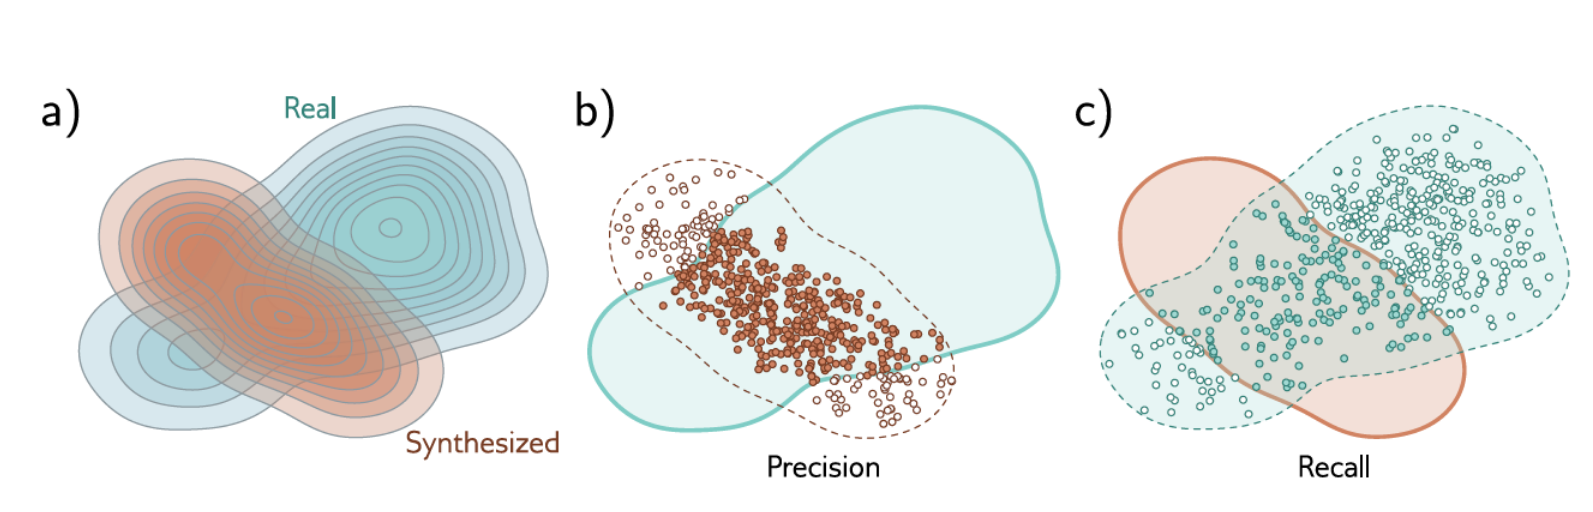
\includegraphics[width=0.8\linewidth]{./img/manifold_precision_recall.png}
\end{figure}



\section{Generative adversarial networks}


\begin{description}
    \item[Generative adversarial network (GAN)] \marginnote{Generative adversarial network (GAN)}
        Given:
        \begin{itemize}
            \item A generator $G(z; \theta)$ that takes an input latent vector $z_i \sim p_\text{lat}(z)$ and produces an image $\hat{x}_j \sim p_\text{gen}(x)$,
            \item A discriminator $D(x; \phi)$ that determines whether $x_i$ is a real image from $p_\text{real}(x)$.
        \end{itemize}
        A generative adversarial network trains both $D$ and $G$ with the aim of making $p_\text{gen}$ converge to $p_\text{real}$.

        \begin{figure}[H]
            \centering
            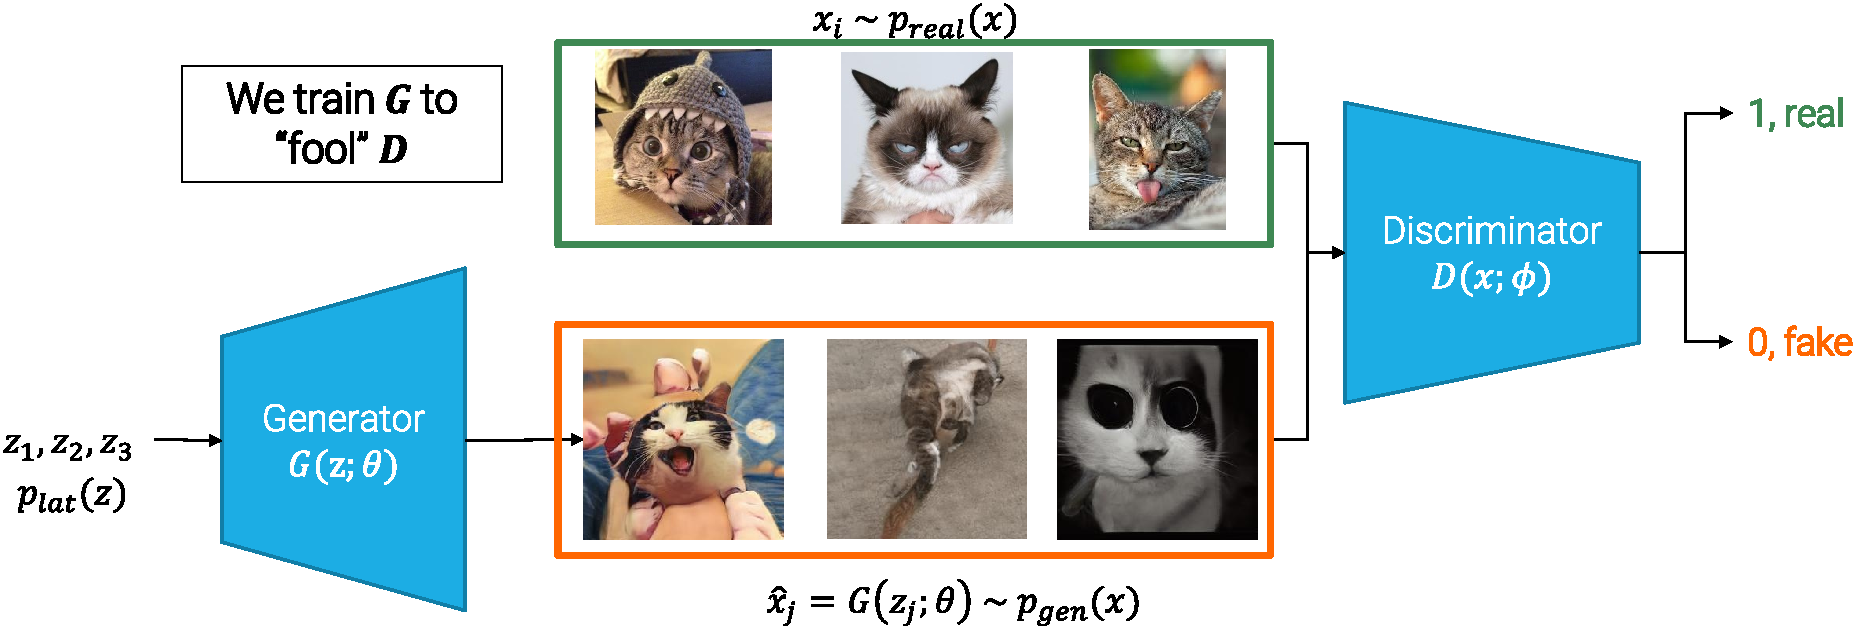
\includegraphics[width=0.8\linewidth]{./img/_gan_flow.pdf}
        \end{figure}


        \begin{description}
            \item[Discriminator loss] \marginnote{Discriminator loss}
                The discriminator solves a binary classification task using binary cross-entropy:
                \[ \mathcal{L}_\text{BCE}(\hat{y}, y) = -y \log(\hat{y}) - (1-y)\log(1-\hat{y}) \]
                As real images always have label $1$ and generated ones always $0$, the optimal parameters are given by the problem:
                \[ 
                    \begin{split}
                        \phi^* &= \arg\min_{\phi} \left\{ 
                            \frac{1}{I} \sum_{i=1}^I \mathcal{L}_\text{BCE}(D(x_i; \phi), 1) + 
                            \frac{1}{J} \sum_{j=1}^J \mathcal{L}_\text{BCE}(D(\hat{x}_j; \phi), 0) 
                        \right\} \\ 
                        &= \arg\min_{\phi} \left\{ 
                            -\frac{1}{I} \sum_{i=1}^I \log \left( D(x_i; \phi) \right) - 
                            \frac{1}{J} \sum_{j=1}^J \log \left( 1- D(\hat{x}_j; \phi) \right) 
                        \right\}
                    \end{split}
                \]
                Therefore, the discriminator loss can be formulated as:
                \[ \mathcal{L}_D(\phi) = - \sum_{i=1}^{I} \log(D(x_i; \phi)) - \sum_{j=1}^{J} \log(1-D(\hat{x}_i; \phi)) \]

            \item[Generator loss] \marginnote{Generator loss}
                The generator aims to fool the discriminator. Its objective is therefore to maximize the loss the discriminator is minimizing:
                \[ \theta^* = \arg\max_\theta \left\{ \min_{\phi} \left\{ 
                    -\frac{1}{I} \sum_{i=1}^I \log \left( D(x_i; \phi) \right) - 
                    \frac{1}{J} \sum_{j=1}^J \log \left( 1- D(G(z_j; \theta); \phi) \right) 
                \right\} \right\} \]
                As the generator only influences the second term, the overall generator loss is:
                \[ \mathcal{L}_G(\theta) = \sum_{j=1}^{J} \log\left( 1 - D(G(z_j; \theta); \phi) \right) \]


            \item[Training]
                Generator and discriminator are trained together in a minimax game as follows:
                \begin{enumerate}
                    \item Sample a batch of latent vectors $z_1, \dots, z_j$ to generate $\hat{x}_1, \dots, \hat{x}_j$.
                    \item Sample a batch of real images $x_1, \dots, x_i$.
                    \item Merge the two batches and optimize for $\mathcal{L}_D(\phi)$ and $\mathcal{L}_G(\theta)$.
                \end{enumerate}
        \end{description}

        \begin{remark}[Optimal discriminator]
            The discriminator loss can be seen as a sum of two expectations (that uses Monte Carlo approximation):
            \[ 
                \begin{split}
                    \mathcal{L}_D(\phi) &= - \frac{1}{I} \sum_{i=1}^{I} \log(D(x_i; \phi)) - \frac{1}{J} \sum_{j=1}^{J} \log(1-D(\hat{x}_i; \phi)) \\
                    &\approx -\mathbb{E}_{x_i \sim p_\text{real}(x)}\left[ \log(D(x_i; \phi)) \right] - \mathbb{E}_{\hat{x}_j \sim p_\text{gen}(x)}\left[ \log(1-D(\hat{x}_j; \phi)) \right] \\
                    &= - \int p_\text{real}(x) \log(D(x; \phi)) + p_\text{gen}(x) \log(1-D(x; \phi)) \,dx
                \end{split}
            \]
            By calling $a = p_\text{real}(x)$, $b = p_\text{gen}(x)$, and $y = D(x; \phi)$, we have that:
            \[ \int a \log(y) + b \log(1-y) \,dx \]
            To obtain the minimum w.r.t. $y = D(x; \phi)$, we have that:
            \[ 
                \begin{split}
                    \frac{\partial}{\partial y}\left[ a \log(y) + b \log(1-y) \right] = 0 
                    &\Rightarrow \frac{a}{y} - \frac{b}{1-y} = 0 \\
                    &\Rightarrow y = \frac{a}{a-b}
                \end{split}
            \]
            Therefore, the optimal theoretical discriminator is:
            \[ D^*(x) = \frac{p_\text{real}(x)}{p_\text{real}(x) + p_\text{gen}(x)} \]
            This makes sense as:
            \begin{itemize}
                \item With a real image ($p_\text{real}(x)$ high) and a bad generator ($p_\text{gen}(x)$ low), the discriminator is able to detect the real image ($D^*(x) \rightarrow 1$).
                \item With a bad generator ($p_\text{real}(x)$ low and $p_\text{gen}(x)$ high), the discriminator is able to detect the generator ($D^*(x) \rightarrow 0$).
                \item With a perfect generator ($p_\text{real}(x)$ and $p_\text{gen}(x)$ are both high), the discriminator is undecided ($D^*(x) \rightarrow 0.5$).
            \end{itemize}
        \end{remark}

        \begin{remark}[Optimal generator]
            By inserting the optimal discriminator into the (full) generator loss, we have that:
            \[
                \footnotesize
                \begin{split}
                    \mathcal{L}_G(x) &= - \int p_\text{real}(x) \log\left(\frac{p_\text{real}(x)}{p_\text{real}(x) + p_\text{gen}(x)}\right) + p_\text{gen}(x) \log\left(1 - \frac{p_\text{real}(x)}{p_\text{real}(x) + p_\text{gen}(x)}\right) \,dx \\
                    &= - \int p_\text{real}(x) \log\left(\frac{p_\text{real}(x)}{p_\text{real}(x) + p_\text{gen}(x)}\right) \,dx - \int p_\text{gen}(x) \log\left(\frac{p_\text{gen}(x)}{p_\text{real}(x) + p_\text{gen}(x)}\right) \,dx \\
                    &= - \int p_\text{real}(x) \log\left({\frac{2}{2}} \frac{p_\text{real}(x)}{p_\text{real}(x) + p_\text{gen}(x)}\right) \,dx - \int p_\text{gen}(x) \log\left({\frac{2}{2}} \frac{p_\text{gen}(x)}{p_\text{real}(x) + p_\text{gen}(x)}\right) \,dx \\
                    &= - \int p_\text{real}(x) \log\left(\frac{{2} p_\text{real}(x)}{p_\text{real}(x) + p_\text{gen}(x)}\right) + {\log\left(\frac{1}{2}\right)} \,dx - \int p_\text{gen}(x) \log\left(\frac{{2} p_\text{gen}(x)}{p_\text{real}(x) + p_\text{gen}(x)}\right) + {\log\left(\frac{1}{2}\right)} \,dx \\
                    &= - \int p_\text{real}(x) \log\left(\frac{2 p_\text{real}(x)}{p_\text{real}(x) + p_\text{gen}(x)}\right) \,dx - \int p_\text{gen}(x) \log\left(\frac{2 p_\text{gen}(x)}{p_\text{real}(x) + p_\text{gen}(x)}\right) \,dx + \log(4)  \\
                    &= - \int p_\text{real}(x) \log\left(\frac{p_\text{real}(x)}{\frac{p_\text{real}(x) + p_\text{gen}(x)}{2}}\right) \,dx - \int p_\text{gen}(x) \log\left(\frac{p_\text{gen}(x)}{\frac{p_\text{real}(x) + p_\text{gen}(x)}{2}}\right) \,dx + \log(4)  \\
                    &= - D_\text{KL}\left( p_\text{real}(x) || \frac{p_\text{real}(x) + p_\text{gen}(x)}{2} \right) - D_\text{KL}\left( p_\text{gen}(x) || \frac{p_\text{real}(x) + p_\text{gen}(x)}{2} \right) + \log(4) \\
                    &= -2 D_\text{JS}\left( p_\text{real}(x) || p_\text{gen}(x) \right) + \log(4)
                \end{split}
            \]
            Therefore, the generator aims to maximize $-2 D_\text{JS}\left( p_\text{real}(x) || p_\text{gen}(x) \right) + \log(4)$. As $D_\text{JS}(\cdot) \geq 0$, the optimal generator aims to achieve $D_\text{JS}(\cdot) = 0$ which happens when:
            \[ p_\text{real}(x) = p_\text{gen}(x) \]
        \end{remark}

        \begin{remark}
            Even though on a theoretical level a perfect discriminator and generator exist, in practice neural networks are finite and it is not clear if the alternating minimization steps converge.
        \end{remark}

        \begin{remark}
            The original GAN only uses fully-connected layers.
        \end{remark}
\end{description}


\subsection{Deep convolutional GAN}

\begin{description}
    \item[Deep convolutional GAN (DCGAN)] \marginnote{Deep convolutional GAN (DCGAN)}
        GAN with a fully-convolutional architecture.

        \begin{figure}[H]
            \centering
            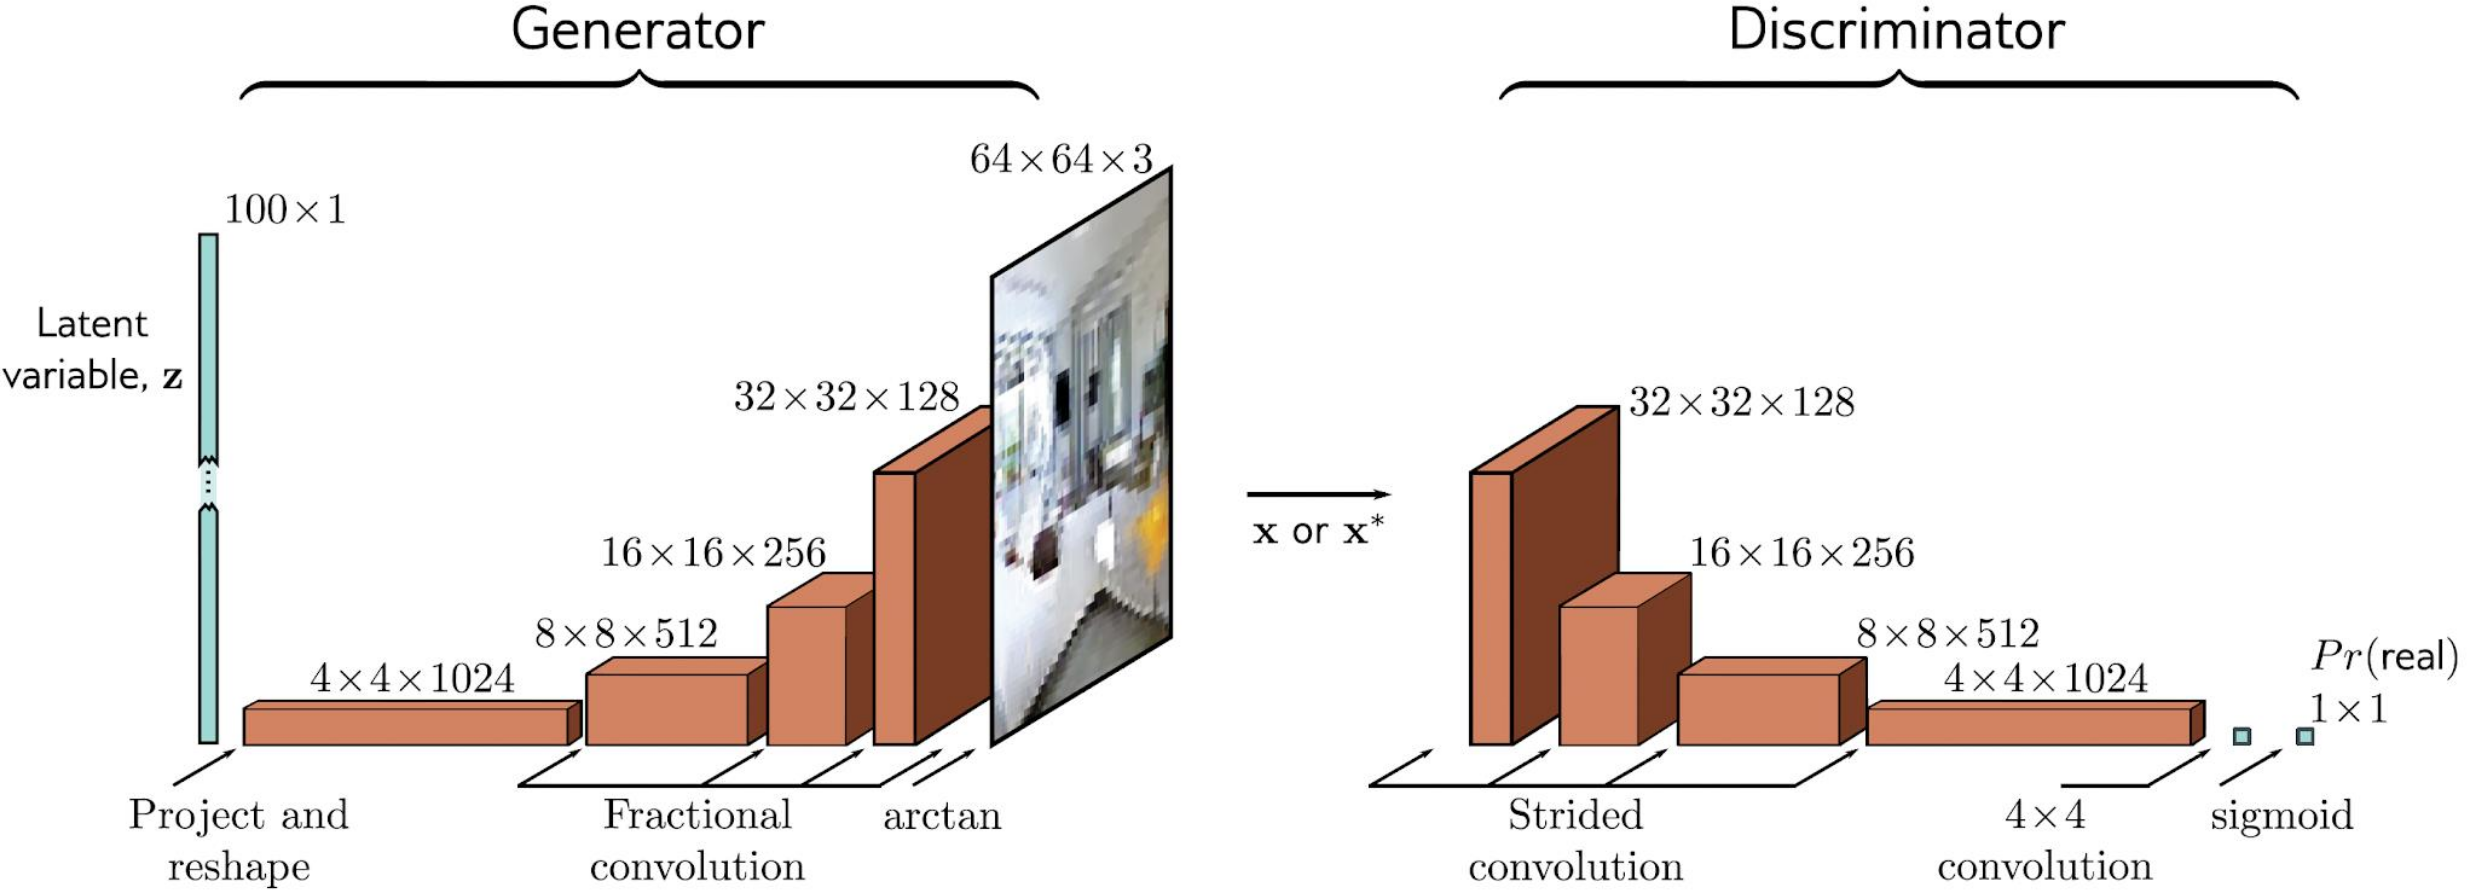
\includegraphics[width=0.6\linewidth]{./img/dcgan.png}
        \end{figure}
\end{description}

\begin{remark}
    The latent space of GANs is well-behaved: directions in the latent space have a meaning.

    \begin{figure}[H]
        \centering
        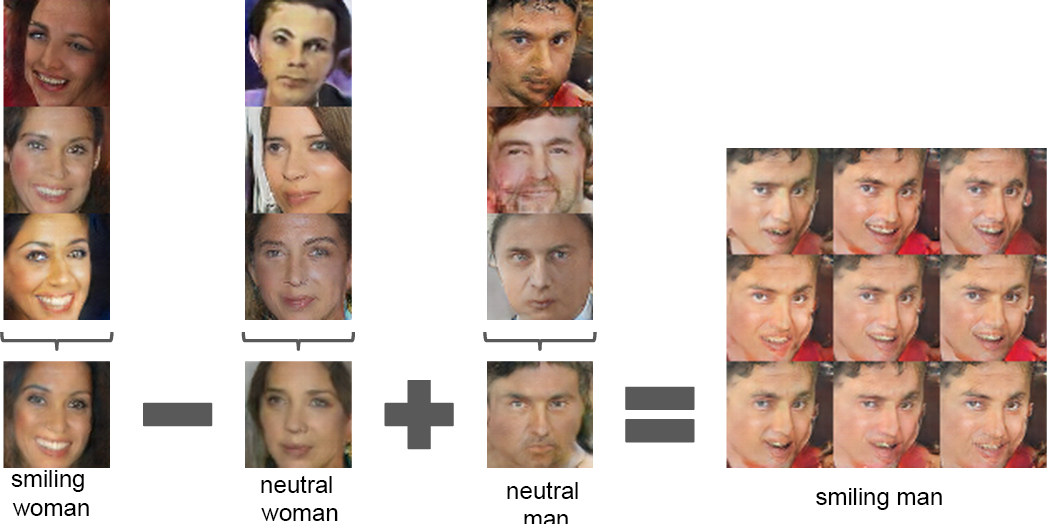
\includegraphics[width=0.5\linewidth]{./img/gan_latent_interpolation.png}
    \end{figure}
\end{remark}

\begin{remark}[Mode dropping/collapse]
    Only some modes of the distribution of the real data are represented by the mass of the generator.

    Consider the training objective of the optimal generator. Its main terms model coverage and quality, respectively:
    \[ 
        \begin{gathered}
            -\frac{1}{I} \sum_{i=1}^I \log \left( D(x_i; \phi) \right) - \frac{1}{J} \sum_{j=1}^J \log \left( 1- D(G(z_j; \theta); \phi) \right) \\
            = - \underbrace{D_\text{KL}\left( p_\text{real}(x) || \frac{p_\text{real}(x) + p_\text{gen}(x)}{2} \right)}_{\text{Coverage}}
            - \underbrace{D_\text{KL}\left( p_\text{gen}(x) || \frac{p_\text{real}(x) + p_\text{gen}(x)}{2} \right)}_{\text{Quality}}
            + \log(4) 
        \end{gathered}
    \]
    The coverage term is high for regions with real images and no generated ones. The quality term is high for regions with generated images and no real ones.

    As the generator only affects the second term (quality), this might be a reason that causes mode collapse.
\end{remark}

\begin{remark}[Disjoint distributions]
    As real and generated images lie in low-dimensional subspaces, it is likely that their distributions are disjoint. The training objective of GANs aims to minimize the JS divergence, which is maximum if the distributions do not overlap causing no significant signal for gradient updates.

    In other words, whenever the generator or discriminator becomes too performant (i.e., the distributions become too different), updates to the other component carry no signal.

    \begin{figure}[H]
        \centering
        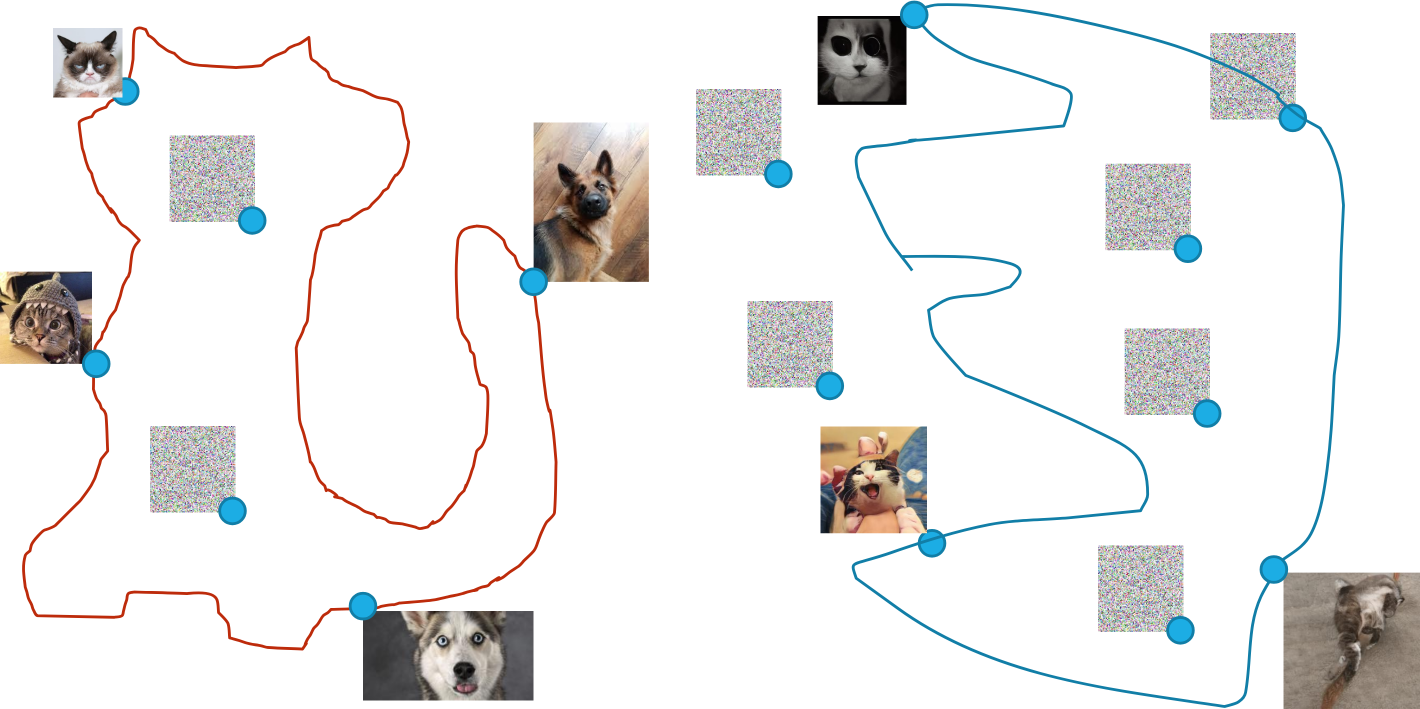
\includegraphics[width=0.7\linewidth]{./img/gan_disjoint.png}
    \end{figure}

    \indenttbox
    \begin{example}
        By freezing the generator while training the discriminator, it takes few epochs for it to achieve near perfect accuracy.
    \end{example}
\end{remark}


\subsection{Wasserstein GAN}

\begin{description}
    \item[Wasserstein GAN (WGAN)] \marginnote{Wasserstein GAN (WGAN)}
        Train a GAN using the Wasserstein distance (i.e., EMD) to compare distributions.

        \begin{remark}
            The Wasserstein distance is meaningful even with disjoint distributions.
        \end{remark}

        \begin{remark}
            It can be shown that the objective is easier to optimize in the dual form of the linear programming formulation.
        \end{remark}
\end{description}


\subsection{Progressive GAN}

\begin{description}
    \item[Progressive GAN (ProGAN)] \marginnote{Progressive GAN (ProGAN)}
        GAN for high-resolution generation with a coarse-to-fine approach. 
        
        \begin{description}
            \item[Training] 
                The network starts as a generator for $4 \times 4$ images and its resolution is incrementally increased.

                \begin{figure}[H]
                    \centering
                    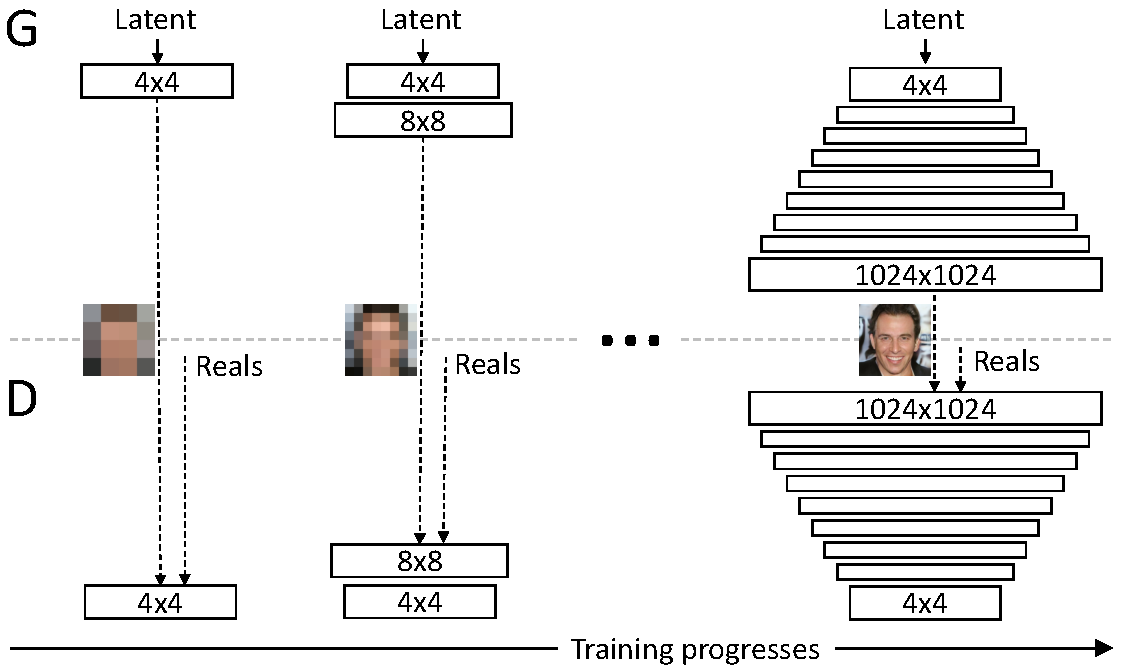
\includegraphics[width=0.65\linewidth]{./img/_progan.pdf}
                \end{figure}

                \begin{description}
                    \item[Layer fade-in] 
                        When moving from an $n \times n$ to $2n \times 2n$ resolution, the following happens:
                        \begin{itemize}
                            \item The generator outputs a linear combination between the $n \times n$ image up-sampled (with weight $1-\alpha$) and the $n \times n$ image passed through a transpose convolution (with weight $\alpha$).
                            \item The discriminator uses a linear combination between the $2n \times 2n$ image down-sampled (with weight $1-\alpha$) and the $2n \times 2n$ image passed through a convolution.
                        \end{itemize}
                        Where $\alpha$ grows linearly from 0 to 1 during training. This allows the network to use old information when the resolution changes and gradually adapt.

                        \begin{figure}[H]
                            \centering
                            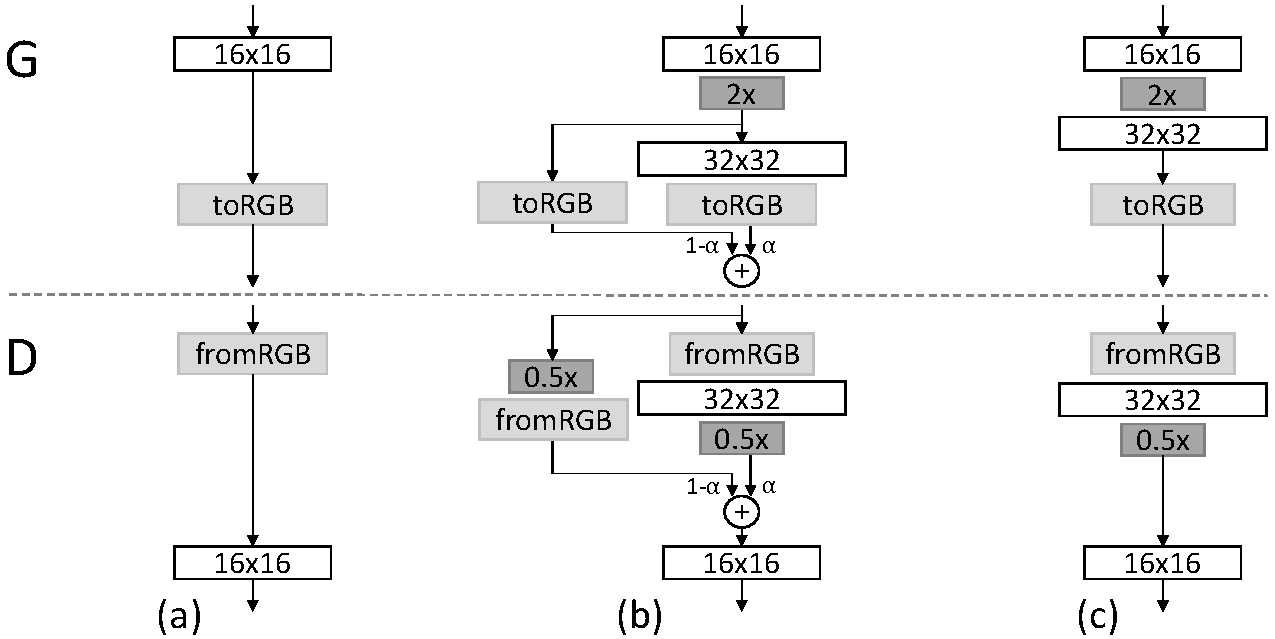
\includegraphics[width=0.7\linewidth]{./img/_progan_fadein.pdf}
                            \caption{
                                \parbox[t]{0.7\linewidth}{
                                    ProGAN fade-in. (a) is the starting resolution. (b) depicts the fade-in process. (c) represents the network at the end of the training process for this resolution (i.e., with $\alpha=1$)
                                }
                            }
                        \end{figure}
                \end{description}
        \end{description}
\end{description}


\subsection{StyleGAN}

\begin{description}
    \item[Instance normalization] \marginnote{Instance normalization}
        Normalize along spatial dimensions only (i.e., there is a mean and variance for every channel of the image and every element of the batch).

        \begin{description}
            \item[Adaptive instance normalization (AdaIN)] \marginnote{Adaptive instance normalization (AdaIN)}
                Given a content $c \in \mathbb{R}^{B \times C \times H \times W}$ and a style $s \in \mathbb{R}^{B \times C \times H \times W}$, AdaIN normalizes $c$ while injecting information from $s$ as follows:
                \[ \sqrt{v_s} \frac{c - \mu_c}{\sqrt{v_c + \varepsilon}} + \mu_s \]
                where $\mu_c \in \mathbb{R}^{B \times C \times 1 \times 1}$ and $v_c \in \mathbb{R}^{B \times C \times 1 \times 1}$ are mean and variance of $c$ and $\mu_s \in \mathbb{R}^{B \times C \times 1 \times 1}$ and $v_s \in \mathbb{R}^{B \times C \times 1 \times 1}$ are mean and variance of $s$.
        \end{description}


    \item[StyleGAN] \marginnote{StyleGAN}
        Network that does the following:
        \begin{enumerate}
            \item Preprocess the input latent vector with fully-connected layers.
            \item Add to the starting constant image (learned during training) some noise.
            \item Pass the current image as the content of AdaIN and use the refined latent vector as the style.
            \item Continue as normal GANs, with AdaIN using the latent vector as style after every convolution.
        \end{enumerate}

        \begin{figure}[H]
            \centering
            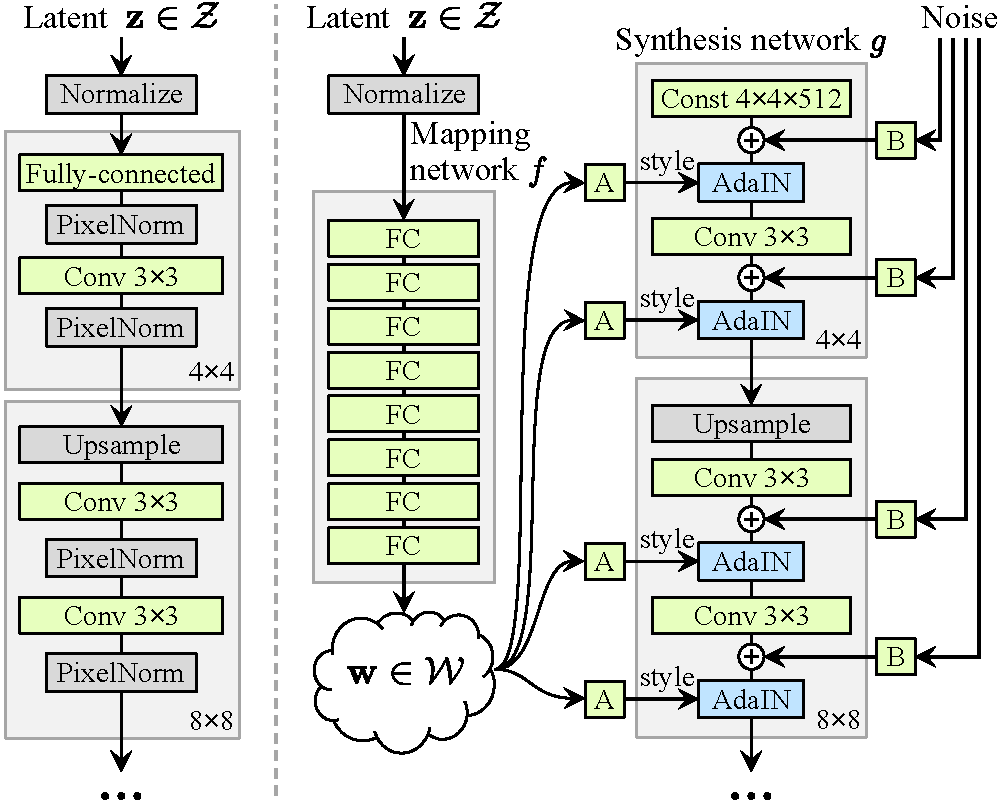
\includegraphics[width=0.4\linewidth]{./img/_stylegan.pdf}
        \end{figure}

        \begin{remark}
            It has been observed that the refined latent representation is more disentangled.
        \end{remark}

        \begin{remark}
            In normal GANs, the latent vector encodes both information on the image to generate and some noise for variability. In StyleGAN, these two aspects are ideally separated.
        \end{remark}
\end{description}

\begin{remark}
    Adversarial losses can also be used in supervised problems (e.g., generate a colored version of a black-and-white image).
\end{remark}